\documentclass[12pt,a4paper]{article}
\usepackage[utf8]{inputenc}
\usepackage[siunitx,american]{circuitikz}
\usepackage{pgfplots}
\usepackage[margin=0.5in]{geometry}
\usepackage{textcomp}
\usepackage[spanish, es-tabla]{babel}
\usepackage{amsmath}
\usepackage{graphicx}
\usepackage[colorinlistoftodos]{todonotes}
\usepackage{amsmath}
\usepackage{tikz}
\usepackage{booktabs}
\usetikzlibrary{arrows}


\usepackage{parskip}
\usepackage{fancyhdr}
\usepackage{vmargin}
\setmarginsrb{3 cm}{2.5 cm}{3 cm}{2.5 cm}{1 cm}{1.5 cm}{1 cm}{1.5 cm}


\pgfplotsset{compat=1.15}

\begin{document}
\section{Ejercicio 3}
\subsection{Introducción}

En esta sección se estudian las corrientes y tensiones de offset de un amplificador operacional. Dichas corrientes no existen en un amplificador operacional
ideal ya que este tiene impedancia infinita de entrada por lo que no fluyen corrientes en sus respectivas entradas. Sin embargo, en un amplificador operacional real 
esta impedancia infinita no existe y entran en juego las corrientes y tensiones de offset que pueden ser perjudiciales en circuitos de alta impedancia. En consecuencia, su análisis previo es sumamente recomendable para un apropiado diseño del
circuito. A continuación, se muestra el modelo del amplificador operacional real.

%modelo del opamp ideal
\begin{figure}[ht]                                                       
    \centering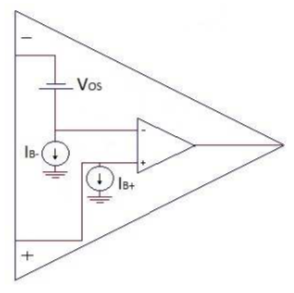
\includegraphics[width=0.4\textwidth, height=5cm]{Figuras/fig_0.png}
     \caption{Modelo del amplificador operacional}
     \label{fig_0}
     \end{figure}



Como se puede observar, se trata del modelo ideal del amplificador operacional con dos fuentes de corrientes adicionales y una fuente de tensión.
Las dos fuentes de corriente representan las corrientes de bias ($I_N$ y $I_P$), mientras que la fuente de tensión representa la tensión de offset $V_{os}$.

Teniendo presente el modelo anterior, es posible poner en estudio a un amplificador operacional para poder determinar las corrientes y tensiones de offset. En esta sección se analiza el
amplificador $OA_2$ que se puede ver en la Figura \ref{circuito_medicion}



\begin{figure}[ht]                                                       
    \centering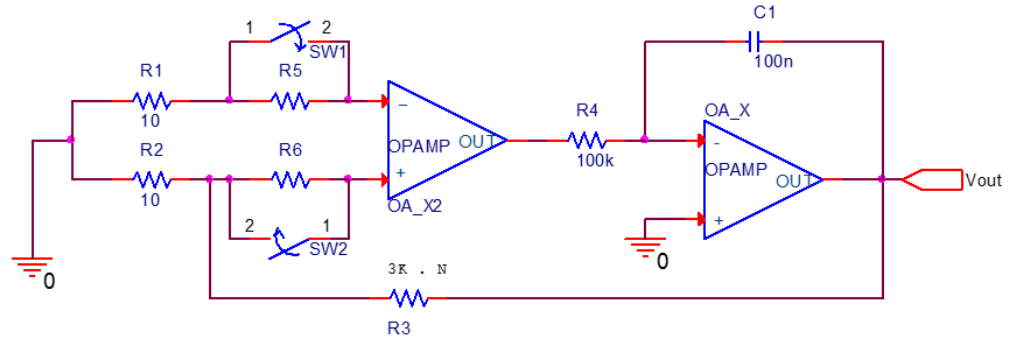
\includegraphics[width=0.8\textwidth, height=5cm]{Figuras/circuito_medicion.png}
     \caption{Circuito de medición de corrientes y tensiones offset}
     \label{circuito_medicion}
     \end{figure}

     
Como se puede observar, se trata de un circuito de medición de corrientes de offset. En este caso se ponen en estudio el comportamiento de los
amplificadores operacionales LF356 y TL081 en el circuito de medición para poder medir sus respectivas corrientes de bias $I_B$, $V_{os}$ y $I_{os}$. Donde $I_B$ y $I_{os}$ se definen como:

\begin{equation} I_{B} = \frac{I_P+I_N}{2} \label{corriente_bias}\end{equation}
\begin{equation} I_{OS} = I_P - I_N \label{corriente_offset}\end{equation}

\subsection{Análisis teórico del circuito}


En primer lugar se estudia teóricamente el circuito de la Figura \ref{circuito_medicion} para comprender como esta compuesto y porque se puede utilizar para medir $I_B$, 
$V_{os}$  y $I_{os}$. Cabe aclarar que el amplificador operacional de interés (que se se quiere medir) es el $OA_2$, mientras que el $OA_1$ sirve para facilitar la medición. Esto se ve mas adelante.   

Para comenzar el análisis, primero se extrae el amplificador operacional $OA_2$ que es el de importancia. El circuito resultante se muestra en la Figura \ref{inverter}.

%Circuito 1
\begin{figure}[ht]                                                       
    \centering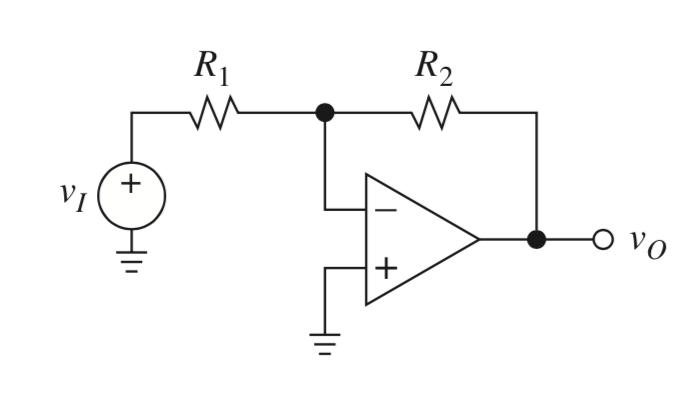
\includegraphics[width=0.5\textwidth, height=5cm]{Figuras/fig_1.png}
     \caption{Amplificador operacional en configuración inversora}
     \label{inverter}
     \end{figure}

Como se puede observar, se trata de un circuito en configuración inversora con realimentacion negativa. Si bien su configuración no es exactamente la misma que se muestra en la Figura \ref{circuito_medicion}, la misma sirve para extraer conceptos que ayudan en la comprensión del circuito.
Su función transferencia, resulta ser:

\begin{displaymath} H(s) = -\frac{A_{vol} R_2}{R_2 + A_{vol} R_1} \end{displaymath}
\begin{displaymath} H_(s) = - \frac{R_2}{R_1 [\frac{R_2}{R_1 A_{vol}}+1]} \end{displaymath}
\begin{displaymath} A_{vol} >> \frac{R_2}{R_1} \end{displaymath}  
\begin{equation}  H_(s) = A_{CL} = - \frac{R_2}{R_1} \label{ganancia_OA_2}\end{equation}

Nótese que la ganancia a lazo abierto $A_{OL} = A_{vol}$, sobre esto se vuelve mas adelante.
Teniendo estos resultados en mente ,si se aplica $V_{in} = 0V$, $V_{out} = 0V$.

Sin embargo, en un amplificador operacional real se deben tener en cuenta $I_N$ $I_P$ y $V_{os}$ como se vio en la Figura \ref{fig_0}. El circuito tomando $V_{in} = 0V$ y considerando $I_N$ y $I_P$ resulta ser el de la 
Figura \ref{fig_2}.

%3
\begin{figure}[ht]                                                       
    \centering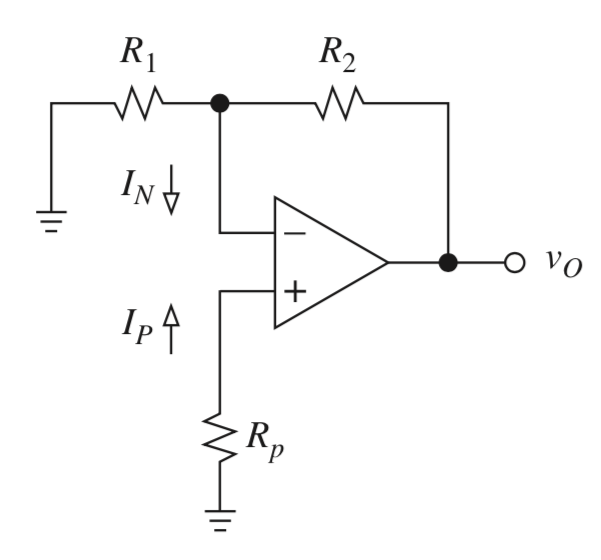
\includegraphics[width=0.5\textwidth, height=5cm]{Figuras/fig_2.png}
     \caption{Circuito considerando $I_N$ y $I_P$}
     \label{fig_2}
     \end{figure}

Este ultimo circuito se puede resolver utilizando el principio de superposición. El resultado es:


\begin{displaymath} V_{out1} = -(1+\frac{R_2}{R_1})R_P I_P \end{displaymath}
\begin{displaymath} V_{out2} = I_N R_2 \end{displaymath}
\begin{displaymath} V_{out} = E_{out} = V_{out1} + V_{out2} \end{displaymath}

Nótese que la tension de salida es llamada $E_{out}$ para ser énfasis que se trata de un error ya que la $V_{out}$ debería ser $0V$. 
Si ahora se considera la existencia de $V_{OS}$, sin considerar  ni $I_{N}$ ni $I_{P}$. El circuito resulta ser el de la Figura \ref{fig_3}.
 

\begin{figure}[ht]                                                       
    \centering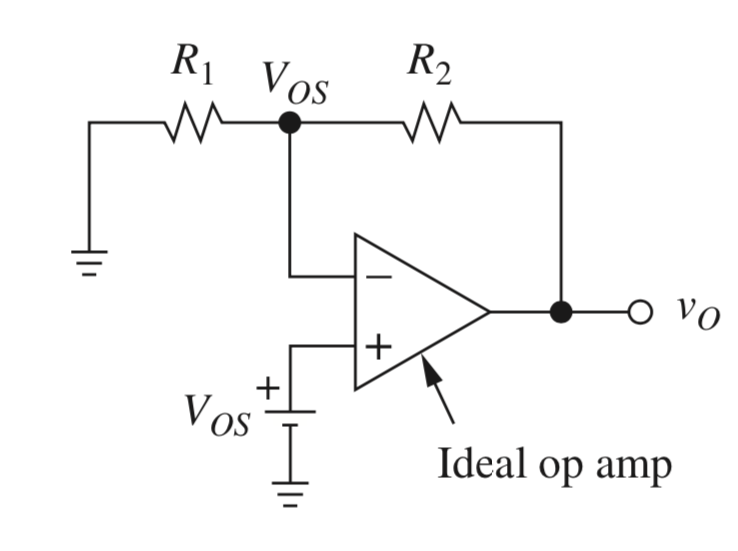
\includegraphics[width=0.5\textwidth, height=5cm]{Figuras/fig_3.png}
    \caption{Circuito considerando $V_{OS}$}
    \label{fig_3}
    \end{figure}


Si se resuelve este ultimo circuito, el resultado es:

\begin{displaymath} V_{out3} = -(1+\frac{R_2}{R_1})V_{OS} \end{displaymath}

Luego, si se suma este ultimo resultado a $V_{out}$:

\begin{equation} V_{out} = -(1+\frac{R_2}{R_1})R_PI_P + I_N R_2 -(1+\frac{R_2}{R_1})V_{OS} \label{V_out_teorico}\end{equation}

Si se tienen en cuenta las definiciones \ref{corriente_bias} y \ref{corriente_offset}, $V_{out}$ resulta ser:

\begin{equation} V_{out} = E_{out} = (1+\frac{R_2}{R_1})[[(\frac{R_1R_2}{R_1+R_2})-R_3]I_B - [(\frac{R_1R_2}{R_1+R_2})+R_P]\frac {I_{OS}}{2}] + (1+\frac{R_2}{R_1})V_{OS} \end{equation}
    Observando esta ultima ecuación, el error se puede disminuir drásticamente si:
\begin{equation} R_3 = \frac{R_1R_2}{R_1+R_2} \label{arreglo_1}\end{equation}
Con este cambio el error queda:
\begin{equation} V_{out} = E_{out} = (1+\frac{R_2}{R_1})(\frac{R_1R_2}{R_1+R_2})I_{OS} + (1+\frac{R_2}{R_1})V_{OS}  \label{error_3}\end{equation}


Gracias a las ecuaciones \ref{error_3} se tiene una relación  de $I_B$, $V_{os}$ y $I_{os}$ con $V_{out}$. Para comprender la magnitud de estos parametros se muestran los valores provistos por los fabricantes
de LF356 y TL081. La tabla \ref{hoja_datos} muestra los valores tipicos y maximos de $I_B$, $V_{os}$ y $I_{os}$.

%METO TABLA
\begin{table}[h!]
    \centering
    \caption{Valores de hojas de datos a 25°C}
    \label{hoja_datos}

    \begin{tabular}{@{}lcc@{}}
        & \multicolumn{1}{l}{Texas Instruments TL081} & \multicolumn{1}{r}{National Semiconductor LF356} \\ \midrule
    \textbf{$V_{OS}$} & Tip: 3mV Max: 10mV      & Tip:3mV Max:10mV             \\
    \textbf{$I_B$}  & Tip: 20pA Max: 400pA    & Tip: 30pA Max:200pA          \\
    \textbf{$I_{OS}$} & Tip: 5pA Max: 100pA     & Tpi: 3nA Max: 50pA          
    \end{tabular}
    \end{table}

    



Si se evaluá \ref{error_3} con los valores típicos de TL081. La señal es muy pequeña para poder ser medida, por lo que se necesita un amplificador de señal. Esto es la funcion de la segunda etapa del circuito que contiene a 
$OA_1$. El objetivo del amplificador operacional $OA_1$ es amplificar la señal de entrada del $OA_2$ para aumentar la precision en la medición de las corrientes y tensiones de offset. La Figura \ref{fig_4} muestra la configuración del amplificador operacional de la segunda etapa.

%4
\begin{figure}[ht]                                                       
    \centering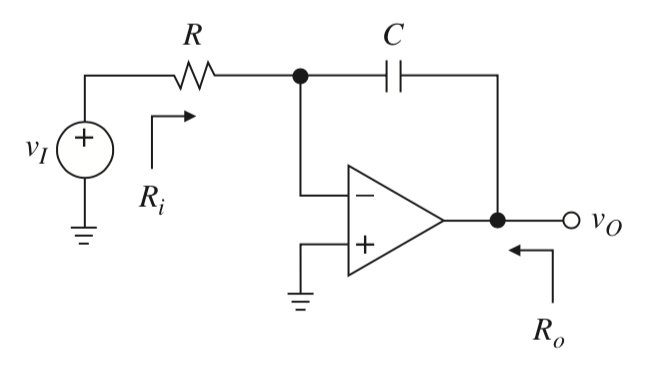
\includegraphics[width=0.5\textwidth, height=5cm]{Figuras/fig_4.png}
     \caption{Amplificador operacional en configuración integradora}
     \label{fig_4}
     \end{figure}


Como se puede observar, el amplificador operacional esta configurado como integrador con una capacitor en la realimentacion. Si se considera su ganancia sin carga finita, su ganancia a lazo cerrado $A_{CL}$ es:

\begin{equation} A_{CL}= \frac{-A_{vol}}{1+SRC A_{vol}}  \label{ganancia_opamp_1} \end{equation}

La función de este amblificador operacional es amplificar la componente DC de la señal de salida $E_{out}$ de $OA_2$ que tiene $f=0Hz$. Entonces, la ecuación 
\ref{ganancia_opamp_1} tiende a estar en configuración a lazo abierto. A $0Hz$ el capacitor $C_{1}$ va a actuar como un circuito abierto, bloqueando cualquier realimentacion
proveniente de la salida de $V_{out}$ cuya frecuencia sea mayor a $f=0Hz$. En esta configuracion, el amplificador operacional es llevado a la saturacion, pero en el caso de configurarlo como en el circuito de medicion en estudio (Figura \ref{circuito_medicion}), esto no es 
un inconveniente. Notese que a este amplificador operacional se lo toma como ideal y no se ve afectado por las corrientes propias de bias ni la su tension de offset. Esta condicion se mantiene a lo largo de toda la seccion. 

Al comprender el funcionamiento de ambas etapas del circuito es posible proseguir al circuito de medición completo. Nuevamente se muestra a continuación.

\begin{figure}[ht]                                                       
    \centering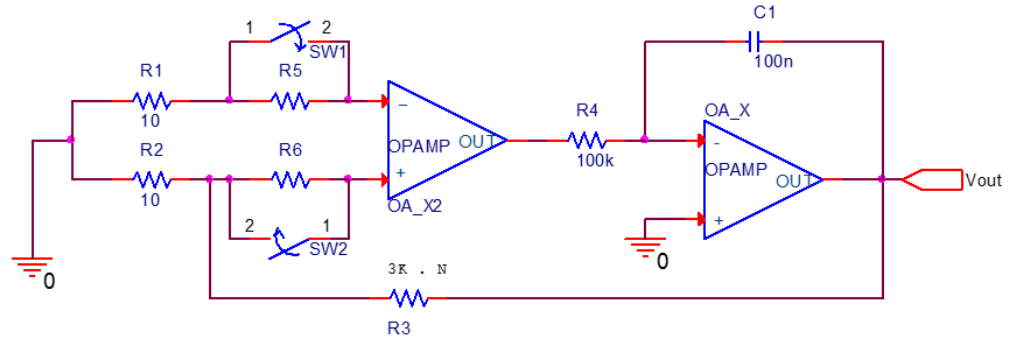
\includegraphics[width=0.8\textwidth]{Figuras/circuito_medicion.png}
     \caption{Circuito de medición de corrientes y tensiones offset}
     \end{figure}

Lo primero que se destaca es que hay una realimentacion desde la segunda etapa a la primera mediante una resistencia $R_3 = 12k\Omega$. Esta realimentacion fuerza la salida de $OA_1$ a tierra e impide la situación de saturación que se destaco
anteriormente.  $OA_2$ tiene conectado a su entrada inversora las resistencias $R_1$ de $10\Omega$ y $R_5$. El circuito cuenta con el switch $SW_1$ que permite poner en corto a $R_5$. Por otro lado,
a la entrada no inversora estan conectados $R_2$ de $10\Omega$, la realimentacion (vista anteriormente) y $R_6$. Como en el caso de $R_5$, $R_6$ también puede
ponerse en corto circuito mediante un el switch $SW_2$. Los valores de $R_5$ y $R_6$ se definirán mas adelante. 

Teniendo esto en cuenta se le agrega al circuito todas las consideraciones vistas anteriormente. El circuito resultante es el de la Figura \ref{medicion_real}.

%5
%circuito de medicion real (le agrego al de medicion, las corrientes de offset y tension de offset)
\begin{figure}[ht]                                                       
    \centering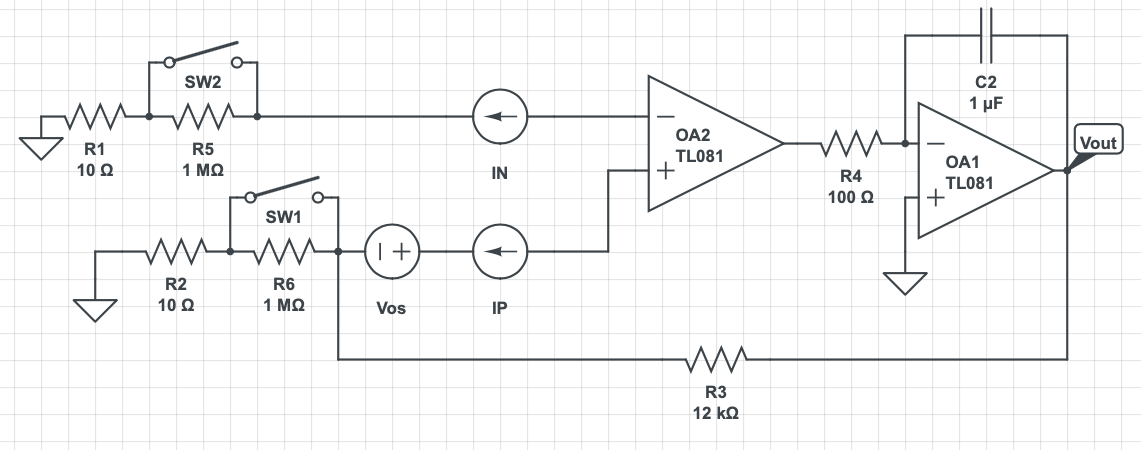
\includegraphics[width=0.8\textwidth]{Figuras/fig_8.png}
     \caption{Circuito de medición real}
     \label{medicion_real}
     \end{figure}

Para resolver el circuito se utiliza el principio de superposición como se hizo anteriormente. En primer lugar se se cierran $SW_1$ y $SW_2$ y se pasivan $I_P$ y $I_N$ de modo que solo quede $V_{OS}$.
Se considera $\Delta V_{R1} = 0$ ya que las corrientes de bias son pequeñas y su valor resistivo también lo es. Con estas condiciones, el circuito se asemeja al visto en la Figura \ref{fig_3} con la salvedad que en este caso se realimenta positivamente. Entonces, resolviendo
mediante el divisor resistivo, se puede obtener una expresión para $V_{out}$

\begin{equation} V_{out1} = -(1 + \frac{R_3}{R_2})V_{OS} \label{ecuacion_Vout_1}\end{equation}

A continuación, se pasiva $V_{OS}$ y $I_N$, se consideran $SW_1$ cerrada y $SW_2$ abierta. También, como en el caso anterior, se desprecia la caída de tension en $R_1$. 
Entonces, si se tiene en cuenta $R_6$ y $I_P$:

\begin{displaymath} V_{N} = 0 \end{displaymath}
\begin{displaymath} V_{P} = - R_6 I_P \end{displaymath}
\begin{displaymath} V_{out} = [1+\frac{R_3}{R_2}] V_{P} \end{displaymath}  
\begin{equation}  V_{out2} = - [1+\frac{R_3}{R_2}] R_6 I_P \label{ecuacion_Vout_2}\end{equation}
 

Nótese que si se considera $V_{OS}$ (no se pasiva) la ecuacion \ref{ecuacion_Vout_1} se suma a la ecuacion \ref{ecuacion_Vout_2} y el resultado es:

\begin{equation} V_{out1} + V_{out2} = -[1 + \frac{R_3}{R_2}]V_{OS} - [1 + \frac{R_3}{R_2}]R_6I_P \label{ecuacion_Vout_3}\end{equation}

Este resultado implica que se puede calcular $I_P$ pasivando a $I_N$, manteniendo las condiciones fijadas anteriormente.

Por otro lado, si se pasiva $V_{OS}$, se cierra $SW_2$ y se abre $SW_1$, se obtiene un resultado semejante al visto anteriormente cuando se trato al amplificador operacional $OA_2$ con realimentacion positiva.
Sin embargo, ahora hay una resistencia $R_5$ en serie con $R_1$. Nuevamente se considera la caída de tension en $R_1$ como nula. El resultado es el siguiente:

\begin{equation} V_{out3} = [1 + \frac{R_3}{R_2}] [-R_5 I_N ]\label{ecuacion_Vout_4}\end{equation}

Nótese que sucede lo mismo que en caso anterior, si considera $V_{OS}$ (no se pasiva) la ecuación \ref{ecuacion_Vout_1} se suma a la ecuación \ref{ecuacion_Vout_4} y el resultado es:

\begin{equation} V_{out1} + V_{out3} = [1 + \frac{R_3}{R_2}] [+R_5 I_N ]  - [1 + \frac{R_3}{R_2}]V_{OS} \label{ecuacion_Vout_5}\end{equation} %R_5 va con menos ??

Este resultado implica que se puede calcular $I_N$ pasivando a $I_P$, siempre y cuando se mantengan las condiciones fijadas anteriormente.

Este conjunto de ecuaciones permite calcular las corrientes de bias y la tension de offset.

\begin{equation} I_{P} = [\frac{V_{out}}{1201} + V_{OS}] \frac{-1}{R_6} (SW_1 cerrado y SW_2 abierto)\label{ecuacion_Ip}\end{equation}
\begin{equation} I_{N} = [\frac{V_{out}}{1201} + V_{OS}] \frac{-1}{R_5} (SW_1 abierto y SW_2 cerrado)\label{ecuacion_In}\end{equation}


A continuación se analiza con mayor profundidad el comportamiento del feedback del circuito y su estabilidad. Recordar que se obtuvieron expresiones para la ganancia a lazo cerrado $A_{CL}$ de ambos amplificadores operacionales 
por separado. Si ahora los consideramos juntos, con la apropiada realimentacion positiva, se puede armar el diagrama de la Figura \ref{diagrama}.

\begin{figure}[h!]                                                       
    \centering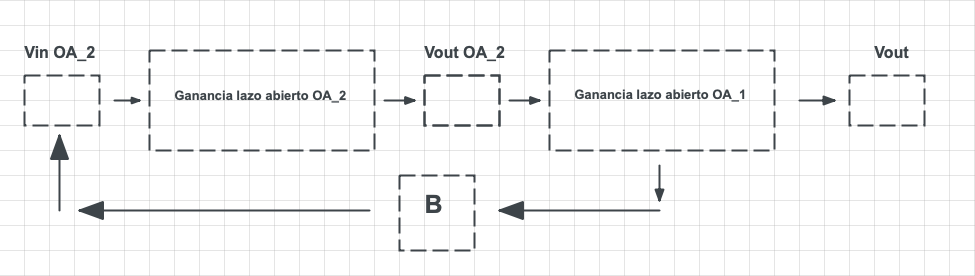
\includegraphics[width=0.8\textwidth]{Figuras/diagrama.png}
     \caption{Diagrama del circuito}
     \label{diagrama}
     \end{figure}

Como se puede ver, es posible agrupar las dos ganancias de los dos amplificadores operacionales. Como se vio anteriormente la ganancia de lazo abierto $A_{OL}$ de $OA_2$ es \ref{ganancia_OA_2} y la ganancia a lazo
cerrado $A_{CL}$ de $OA_1$ es \ref{ganancia_opamp_1}. Luego si las unimos, como se ve en el diagrama, la ganancia a lazo abierto del sistema $A_{OL}$ es:

\begin{equation} A_{OL}= \frac{-A_{vol}^2}{1+SRC A_{vol}}  \label{ganancia_abierto_sistema} \end{equation}

Al estar el sistema realimentado positivamente, la funcion transferencia del sistema es:  
\begin{equation} H (s) = \frac{A_{vol}}{1-A_{vol}\beta} \label{transferencia_sistema_1}  \end{equation}
Si se introduce la ecuación \ref{ganancia_abierto_sistema} a la ecuación \ref{transferencia_sistema_1}, se obtiene:

\begin{equation} H (s) = \frac{-1}{\frac{1}{A_{vol^2}}+\beta}\frac{1}{\frac{s}{(1+A_{vol}^2\beta)RC A_{vol}}+1} \label{transferencia_sistema_2}  \end{equation}

si $A_{vol}^2 \beta >> 1 $  y se considera $A_{vol}$ con el modelo de polo dominante $A_{vol} = \frac{A_0}{\frac{S}{\omega_P}+1}$, la funcion trasferencia del sistema es:

\begin{equation} H (s) = \frac{-1}{\beta} \frac{1}{S^2\frac{RC}{\omega_P A_0 \beta} + \frac{S R C}{A_0 \beta} +1 } \label{transferencia_sistema_3}  \end{equation}

$\beta$ es la ganancia de realimentacion del circuito y como se vio en \ref{ecuacion_Vout_1}:

\begin{equation} \beta =  \frac{1}{1+ \frac{R_3}{R_2}} = \frac{1}{1201} \label{beta}  \end{equation}

\ref{transferencia_sistema_3} permite analizar el sistema en AC. Como se puede obtervar, la expresion de la trasferencia del sistema se asemeja a la de un pasa bajos. Donde:


\begin{displaymath} \omega_0 = \sqrt{\frac{\omega_P A_{0} \beta}{R_4 C_1}} \end{displaymath}
\begin{displaymath} \epsilon = \frac{R_4 C_1 \omega_0}{A_0 \beta 2} \end{displaymath}

Y sus polos son:
\begin{displaymath} S_1 = -\omega_0 \epsilon + \sqrt{\epsilon^2 + 1} \end{displaymath}
\begin{displaymath} S_2 = -\omega_0 \epsilon - \sqrt{\epsilon^2 + 1} \end{displaymath}

Si se evaluan estas expresione con los valores de las frecuencias de corte $f_0$ que proveen los fabricantes de ambos amplificadores operacionales (del orden de los $\Omega$ ) se llega a la conculusion que los polos 
se ubican en el simiplano negativo por lo que el sistema es estable. 

Se puede hacer el mismo analisis con las terminales de los amplificadores operacionales invertidos. Por supuesto que la funcion trasferencia del sistema tendra cambios. Si se invierte $OA_1$, la ganancia a lazo abierto del sistema $A_{OL}$ y la ganancia del feedback $\beta$ son:

\begin{displaymath}  A_{OL}= \frac{+A_{vol}^2}{1-SRC A_{vol}}  \end{displaymath}
\begin{displaymath}  \beta =  \frac{1}{1+ \frac{R_3}{R_2}} = \frac{1}{1201}  \end{displaymath}

Si tambien se invierten las terminales del $OA_2$, el feedback sera negativo y los resultados son:
\begin{displaymath}  A_{OL}= \frac{+A_{vol}^2}{1-SRC A_{vol}}  \end{displaymath}
\begin{displaymath}  \beta =  -\frac{1}{1+ \frac{R_3}{R_2}} = \frac{1}{1201}  \end{displaymath}

\subsection{Mediciones}
Las mediciones se realizaron con el osciloscopio sobre una placa PSB tomando $R_5 = 1M\Omega$ y $R_6 = 1M\Omega$. Se utilizaron capacitares de desacople de $100nF$ y las resistencias indicadas en el circuito de la Figura \ref{circuito_medicion}.
Cabe destacar que para las mediciones se realizaron cuatro combinaciones. Es decir, se alternaron los amplificadores operacionales en las posiciones $OA_1$ y $OA_2$ para analizar como se comportan. 


\subsubsection{Medicion de $V_{OS}$}

Antes de realizar la correspondiente medición de $V_{OS}$, se calcula la respectiva propagación de errores.  A continuación se muestra su desarrollo:

\begin{displaymath} |V_{out1}| = [1 + \frac{R_3}{R_2}]V_{OS} \end{displaymath}
\begin{displaymath} V_{OS} = \frac{R_2}{R_2 + R_3} V_{out1} \end{displaymath}
\begin{displaymath} si R_3 >> R_2 \end{displaymath}  
\begin{displaymath} V_{OS} = \frac{R_2}{R_3} V_{out1} \end{displaymath} 
\begin{displaymath} V_{OS} = f(R_2,R_3) \end{displaymath} 
\begin{displaymath} \Delta V_{OS} = [|\frac{\delta f}{\delta R_2}| \Delta R_2 + |\frac{\delta f}{\delta R_3}| \Delta R_3 ] V_{out1} \end{displaymath} 
\begin{displaymath} \Delta V_{OS} = [\frac {\Delta R_2} { R_3} + \frac{R_2 \Delta R_3 }{R_3^2}] V_{out1} \end{displaymath} 

Nótese que se tomo $R_3 >> R_2$ ya que $R_3 = 1M\Omega $ y $R_2 = 10\Omega$. Ademas esto implica que cuento mas grande sea $R_3$ menor sera el error cometido al medir $V_{OS}$.  

Para medir $V_{OS}$ se debe cerrar $SW_1$ y $SW_2$ como se determino anteriormente. Con esta condición se mide $V_{out}$ y luego, con la ecuación \ref{ecuacion_Vout_1}, se calcula $V_{out}$. Los resultados obtenidos se detallan en la tabla \ref{table2}

\begin{table}[h!]
    \centering
    \caption{Mediciones con $SW_1$ y $SW_2$ cerrados}
    \label{table2}
    \begin{tabular}{@{}ccccc@{}}
    
    \textbf{}           & \textbf{$OA_2$} & \textbf{$OA_1$} & \textbf{$V_{out}(mV)$} & \textbf{$V_{os}$} \\ \midrule
    \textbf{Medición 1} & LF356          & LF356          & -179              &  0.149            \\
    \textbf{Medición 2} & LF356          & TL081          & -184              &  0.153            \\
    \textbf{Medición 3} & TL081          & LF356          & 382,2             &  -0.318            \\
    \textbf{Medición 4} & TL081          & TL081          & 382               &  -0.318            \\ 
    \end{tabular}
\end{table}


\subsubsection{Medicion de $I_{P}$}

Para calcular $I_{P}$ se debe abrir $SW_2$ y mantener cerrado $SW_1$  Al realizar esta acción se observo una oscilación en el circuito impidiendo poder obtener una medición. Esta oscilación es el ruido de linea de 50 Hz que es amplificado por la configuración del circuito.
Esta amplificación del ruido se superpone con $V_{out} = V_{out1} + V_{out2}$ y resulta ser un problema. Para solucionarlo se decidió cambiar al capacitor por uno mas grande. 
Como se discutió anteriormente, el amplificador operacional $OA_1$ tiene una función trasferencia de un pasa bajos y un capacitor "chico" deja pasar un rango de señales mas amplio que un capacitor "grande". Luego si se aumenta el valor del capacitor $C_1$, el polo se 
ubicara en frecuencia mas bajas, filtrando mejor las señales de alta frecuencia. Se prosiguió a cambiar el capacitor $C_1$ a $1\mu F$. Con este cambio se observo una mejora en la señal de salida. Sin embargo, se siguio viendo una oscilacion de 50 Hz. Se prosiguio a cambiar $R_5$ y $R_6$ a distintos
valores pero se siguió observando una oscilacion. En ciertas configuraciones la salida se aproximo a una señal triangular. Ademas se probaron valores de resistencias bajos respecto a los valores iniciales de $R_5$ y $R_6$ como $100\Omega$. Esto se hizo ya que para valores altos de resistencia de
entrada, como lo es $1M\Omega$, el nivel de ruido es mayor. Esto se debe a que si se modela al ruido como una fuente con una resistencia en serie, se forma un divisor resistivo y al ser alto el valor de resistencia de entrada, la salida del divisor es alta afectando al circuito. Sin embargo, al cambiar 
$R_5$ y $R_6$ por valores del orden de los $\Omega$, no es posible medir las corrientes de bias ya que no se puede percibir el cambio de $V_{out}$ al variar $SW_1$ y $SW_2$. En consecuencia se desidio utilizar las resistencias de valor $1M\Omega$ a pesar del ruido y se utilizo la funcion average del osciloscopio
para medir $V_{out}$.
Teniendo todo esto en consideración y con el uso de la \ref{ecuacion_Ip} se obtuvieron los siguientes resultados:


\begin{table}[h!]
    \centering
    \caption{Mediciones con $SW_1$ cerrado y $SW_2$ abierto}
    \label{table3}
    \begin{tabular}{@{}ccccc@{}}
    \textbf{}           & \textbf{$OA_2$} & \textbf{$OA_1$} & \textbf{$V_{out} (mV)$} & \textbf{$I_P$ (pA)} \\ \midrule
    \textbf{Medición 1} & LF356          & LF356          & -130              & -40.799             \\
    \textbf{Medición 2} & LF356          & TL081          & -142              &  -34.970            \\
    \textbf{Medición 3} & TL081          & LF356          & 260              &  101.498            \\
    \textbf{Medición 4} & TL081          & TL081          & 274              & 89.925             \\ 
    \end{tabular}
\end{table}


Cabe aclarar que la Tabla \ref{table2} tiene los resultados con el nuevo capacitor y estos resultados ($V_{OS}$) son utilizados para completar la tabla \ref{table3}. 
En la Figura \ref{medicion} se puede observar la oscilación anteriormente mencionada al abrir $SW_1$. 

\begin{figure}[h!]                                                       
    %\centering\includegraphics[width=0.8\textwidth]{circuito1_ej3.png}
     \caption{$V_{out}$ al abrir $SW_1$}
     \label{medicion}
     \end{figure}



\subsubsection{Medicion de $I_{N}$}


Finalmente se calculo $I_N$ abriendo $SW_1$ y cerrando $SW_2$. El inconveniente de oscilación también se vio replicado en esta medicion, se prosiguió de la misma manera que al medir $I_P$.  
Los resultados fueron los siguientes:

\begin{table}[ht]
    \centering
    \caption{Mediciones con $SW_1$ abierto y $SW_2$ cerrado}
    \label{table4}
    \begin{tabular}{@{}ccccc@{}}
    \textbf{}           & \textbf{$OA_2$} & \textbf{$OA_1$} & \textbf{$V_{out}$} & \textbf{$I_N$} \\ \midrule
    \textbf{Medición 1} & LF356          & LF356          & -159              &  -16.652            \\
    \textbf{Medición 2} & LF356          & TL081          & -160              &  -19.983            \\
    \textbf{Medición 3} & TL081          & LF356          & 356,6              &  26.3114            \\
    \textbf{Medición 4} & TL081          & TL081          & 350              &  21.648            \\ 
    \end{tabular}
\end{table}


\subsubsection{Calculo de $I_{OS}$ y $I_B$}

Con los resultados obtenidos en las tablas \ref{table2}, \ref{table3}, \ref{table4} se puede calcular $I_{OS}$ y $I_B$ siguiendo las ecuaciones \ref{corriente_offset} y \ref{corriente_bias} respectivamente. La siguiente tabla muestra dichos resultados:


\begin{table}[ht]
    \centering
    \caption{$V_{OS}$,$I_{OS}$ y $I_B$ obtenidos}
    \label{table5}
    \begin{tabular}{@{}cccccc@{}}
    \textbf{}           & \textbf{$OA_2$} & \textbf{$OA_1$} & \textbf{$V_{OS} (mV)$}   & \textbf{$I_{OS} (pA)$} & \textbf{$I_B (pA)$} \\ \midrule
    \textbf{Medición 1} & LF356          & LF356      & 0.149                          & 24.146                 & 28.726             \\
    \textbf{Medición 2} & LF356          & TL081      & 0.153                          & 14.987                 & 27.477                  \\
    \textbf{Medición 3} & TL081          & LF356      & -0.318                         & 75.187                 & 63.905                  \\
    \textbf{Medición 4} & TL081          & TL081      & -0.318                         & 68.276                 & 55.786                  \\ 
    \end{tabular}
\end{table}


\subsubsection{Analisis de resultados}
Si se comparan los resultados obtenidos en la tabla \ref{table5} con los datos provistos por los fabricantes (ver Tabla \ref{hoja_datos}), se pueden sacar las siguientes conclusiones. Se puede decir que, a pesar de 
ser un circuito dificultoso para medir, los resultados fueron satisfactorios. En las cuatro mediciones realizadas, los valores de $I_{OS}$ y $I_B$ entraron en los rangos deseados (entre el valor típico y máximo) mientras 
que los valores obtenidos de $V_{OS}$ esta por debajo de los valores típicos. Esto se puede deber a varias razones. En primer lugar, al medir $V_{out}$ con la herramienta del osciloscopio average, el error se incrementa. También, cabe destacar, que
los valores provistos por el fabricante son medidos en un ambiente controlado a $25 °C$. Esta condición no fue cumplida al momento de obtener las mediciones y esa es otra razón por la cual las mediciones de $V_{OS}$ no entran en los rangos deseados.   

\subsection{Circuito de compensación externo}
El objetivo de esta seccion es investigar los circuitos de compensacion externos del LT081 y LF356 para reducir la tension de offset de dichos amplificadores operacioneales.
Para comenzar con el LF356, segun la hoja de datos el cicuito externo de compensacion es el siguiente: 

\begin{figure}[ht]                                                       
    \centering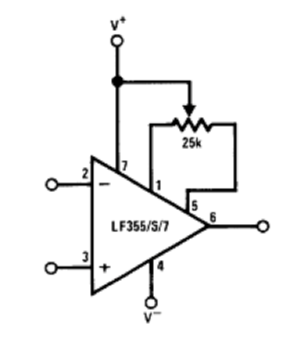
\includegraphics[width=0.5\textwidth, height=5cm]{Figuras/fig_6.png}
     \caption{Circuito de compensación de LF356}
     \label{compensacion_LF356}
     \end{figure}

Como se puede observar, el circuito cuenta con un preset de $25K\Omega$ conectado a $+V_{CC}$. El circuito de compensacion del TL081 es el 
de la Figura \ref{compensacion_LT081}.


\begin{figure}[h!]                                                       
    \centering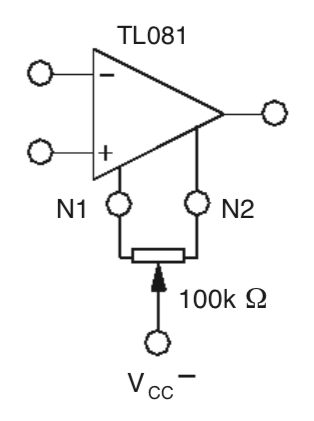
\includegraphics[width=0.5\textwidth, height=6cm]{Figuras/fig_7.png}

    \caption{Circuito de compensación de LT081}
     \label{compensacion_LT081}
     \end{figure}

 

El circuito muestra, que a diferencia del LF356, el fabricante recomienda un preset de $100k\Omega$ conectado a $-V_{CC}$

\end{document}

